\documentclass[sigconf]{acmart}

\usepackage{booktabs} % For formal tables
\usepackage{CJK}
\usepackage{ctex}
\usepackage{color}
\usepackage{graphicx}
\usepackage{amssymb}
\usepackage{amsmath}
\usepackage{amsthm}
\usepackage{booktabs}


\usepackage{fancyhdr}
\usepackage{extramarks}
\usepackage{amsfonts}
\usepackage{tikz}
\usepackage[plain]{algorithm}
\usepackage{algpseudocode}
\usepackage{listings}

% Copyright
\setcopyright{none}

%Conference
\acmConference{Data Communication}{May 2018}{Nanjing, China} 
%\acmYear{2018}
%\copyrightyear{2018}

%\acmPrice{15.00}


\begin{document}
\begin{CJK}{UTF8}{song}

\title{数据通信课外作业}
%\titlenote{Produces the permission block, and copyright information}
%\subtitle{Extended Abstract}

\author{徐子恒 161160037, 赖伟 161250052}
%\authornote{Note}$  $
\orcid{1234-5678-9012}
\affiliation{%
  \institution{计算机科学与技术系}
}
\email{161160037@smail.nju.edu.cn,  161250052@smail.nju.edu.cn}

% The default list of authors is too long for headers}
%\renewcommand{\shortauthors}{F. Lastname et al.}


\begin{abstract}
智能手机已经成为了人们生活中必不可少的电子移动设备,但是应用的高能耗导致智能手机的续航始终是一个难以克服的挑战。网页浏览器是智能手机中最核心的应用之一。但因为移动浏览器在性能上进行了大量优化,给耗电的移动设备带来了巨大的负担。因此,我们的目的是减少智能手机加载网页所消耗的能源,同时最好不会增加页面加载时间和损害用户体验。
\end{abstract}

%
% The code below should be generated by the tool at
% http://dl.acm.org/ccs.cfm
% Please copy and paste the code instead of the example below. 
%
\begin{CCSXML}
<ccs2012>
 <concept>
  <concept_id>10010520.10010553.10010562</concept_id>
  <concept_desc>Computer systems organization~Embedded systems</concept_desc>
  <concept_significance>500</concept_significance>
 </concept>
 <concept>
  <concept_id>10010520.10010575.10010755</concept_id>
  <concept_desc>Computer systems organization~Redundancy</concept_desc>
  <concept_significance>300</concept_significance>
 </concept>
 <concept>
  <concept_id>10010520.10010553.10010554</concept_id>
  <concept_desc>Computer systems organization~Robotics</concept_desc>
  <concept_significance>100</concept_significance>
 </concept>
 <concept>
  <concept_id>10003033.10003083.10003095</concept_id>
  <concept_desc>Networks~Network reliability</concept_desc>
  <concept_significance>100</concept_significance>
 </concept>
</ccs2012>  
\end{CCSXML}

\ccsdesc[500]{Computer systems organization~Embedded systems}
\ccsdesc[300]{Computer systems organization~Redundancy}
\ccsdesc{Computer systems organization~Robotics}
\ccsdesc[100]{Networks~Network reliability}

% We no longer use \terms command
%\terms{Theory}

\keywords{关键词}


\maketitle

\section{Background} %注意 这里目前支持英文
背景介绍

\section{Problem}
问题描述

\section{Overview}
已有工作分类,介绍

\subsection{class 1}
有一些工作从用户的角度 ...



方法结构图,如图 \ref{fig:tasks} 
\begin{figure}[htbp]
\centering
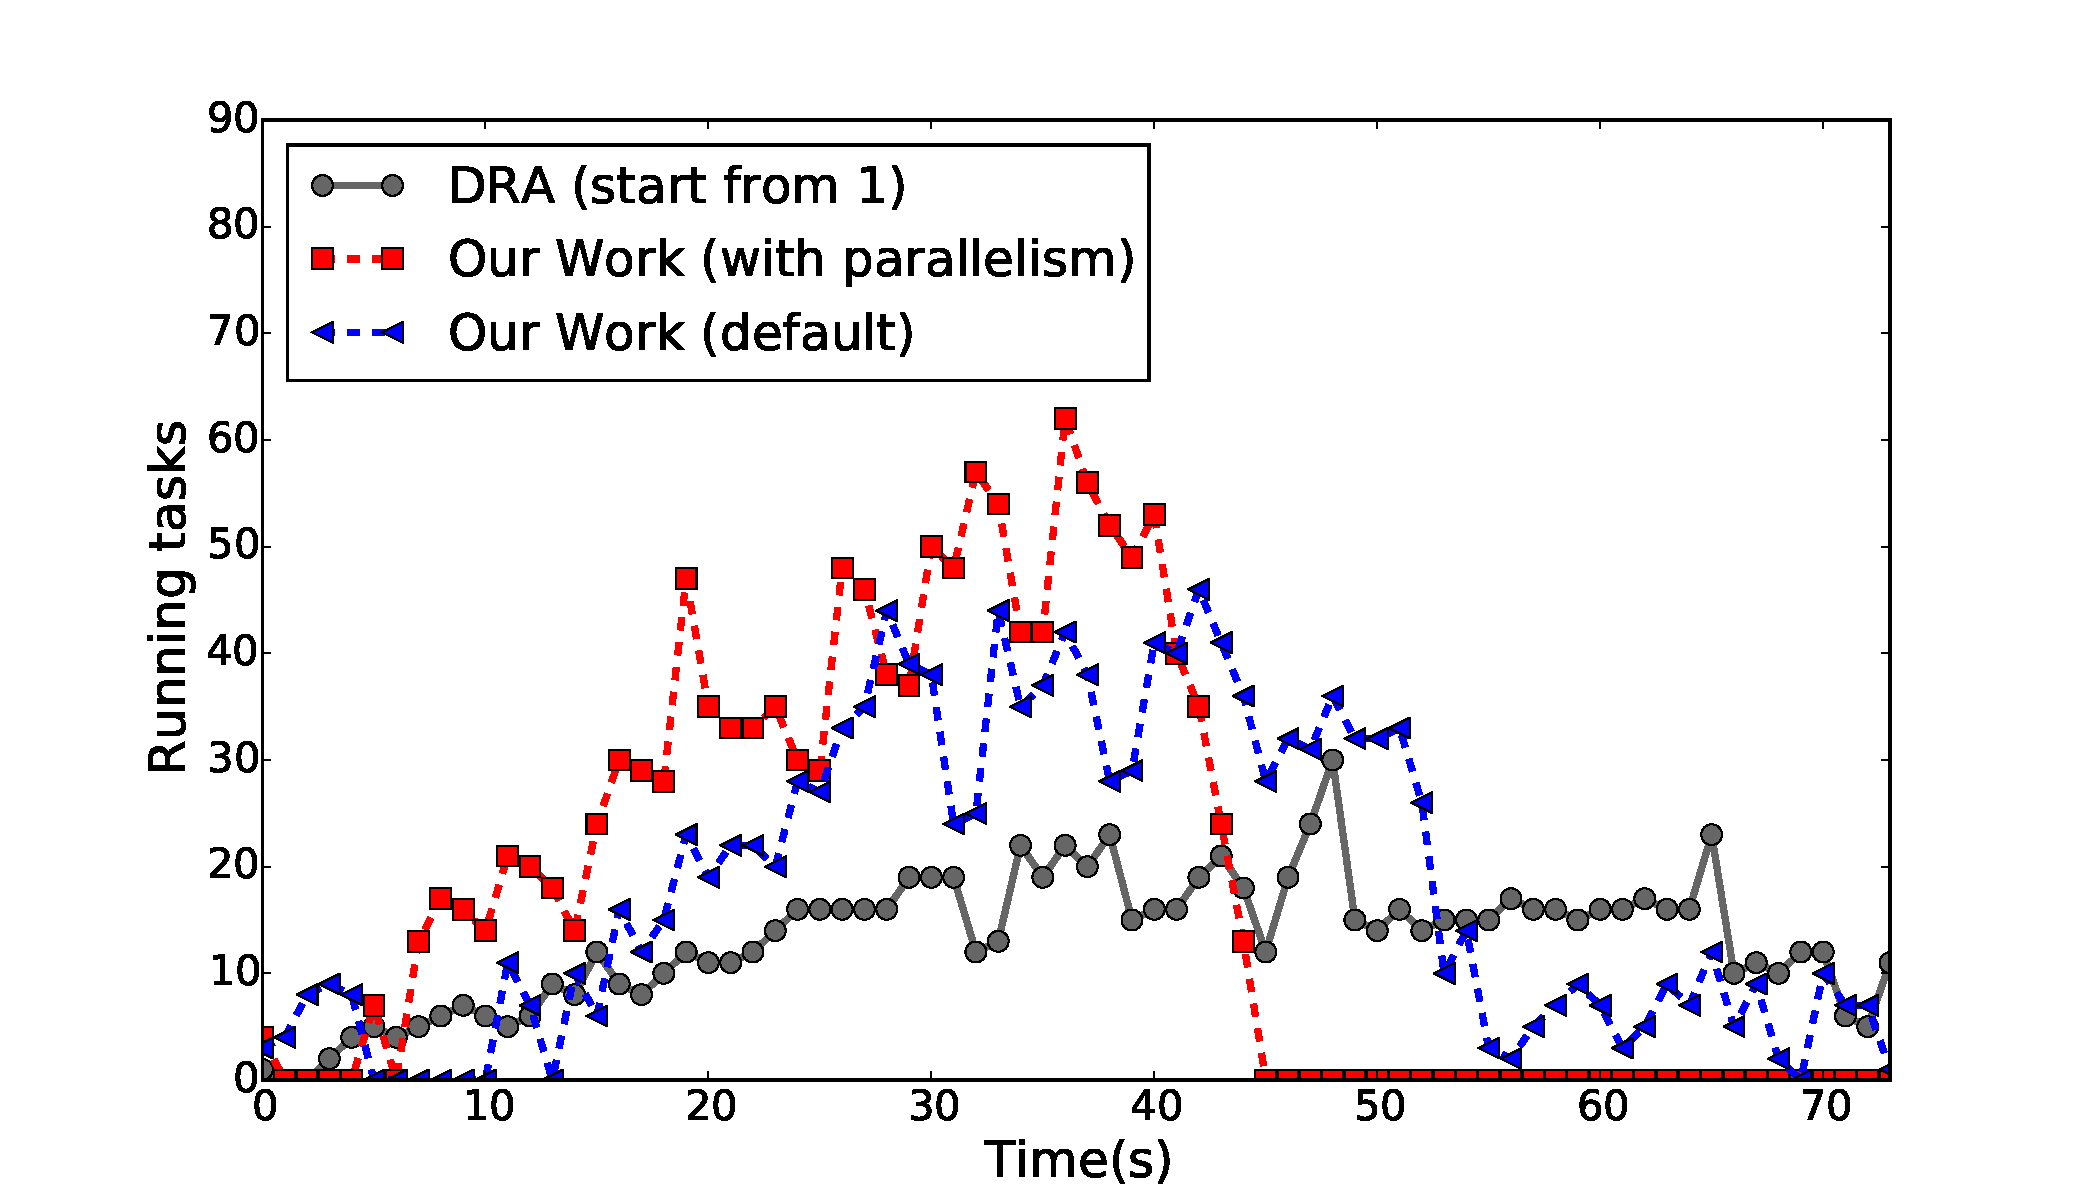
\includegraphics[width=3.4in]{./figure/tasks.pdf}
\caption{Number of Running Tasks}\label{fig:tasks}
\end{figure}

\subsection{class 2}
还有一些工作从环境的角度 ...

\section{conclusion}
结论

注意:参考文献必须完整


\bibliographystyle{ACM-Reference-Format}
\bibliography{sigproc} 

\end{CJK}{UTF8}{song}
\end{document}
